\chapter{The Standard Model of Particle Physics}
\label{c:the_standard_model}

\section{Introduction}
\label{s:standard_model_intro}

The Standard Model (SM) is the name given to the theory developed during the course of the \nth{20} century
that describes the elementary particles that make up all known, observable matter and the three fundamental
forces by which they interact (electromagnetic, weak and strong). The SM does not, however, describe the
gravitational force as it is not known how to model it mathematically at a quantum scale. The SM puts forward
twelve fermions, with a spin quantum number of 1/2, as the matter particles. These are split into two groups
of six quarks and six leptons, all of which are split into three generations. The six quarks are classified
according to their charge and flavour: up, down, charm, strange, top and beauty quarks. The leptons are in
turn classified according to their charge and flavour: electron, muon or tau leptons, together with their
corresponding neutrinos. Neutrinos, although originally thought to be massless, are now believed to carry mass
due to the observation of the oscillation of neutrinos between different flavours.
Table~\ref{tab:standard_model} shows these particles of the Standard Model in their respective generations.
All of these particles have a respective antiparticle which has identical quantum numbers except opposite
electric charge.

\begin{table}[hbth]
\centering
\begin{tabular}{lllll}
\hline
Generation & Flavour & Charge / $e$ & Spin & Mass /\MeV \\
\hline
\hline
\multicolumn{5}{c}{\textbf{Leptons}} \\
\hline
\multirow{2}{*}{I} & electron (e) & -1 & $\frac{1}{2}$ & 0.511 \\
 & electron neutrino ($\nu_{e}$) & 0  & $\frac{1}{2}$ & 0 \\
\hline
\multirow{2}{*}{II} & muon ($\mu$) & -1 & $\frac{1}{2}$ & 105.66 \\
 & muon neutrino ($\nu_{\mu}$) & 0 & $\frac{1}{2}$ & 0 \\
\hline
\multirow{2}{*}{III} & tau ($\tau$) & -1 & $\frac{1}{2}$ & 105.66 \\
 & tau neutrino ($\nu_{\tau}$) & 0 & $\frac{1}{2}$ & 0 \\
\hline
\hline
\multicolumn{5}{c}{\textbf{Quarks}} \\
\hline
\multirow{2}{*}{I} & up (u) & $+\frac{2}{3}$ & $\frac{1}{2}$ & $2.3^{+0.7}_{-0.5}$ \\
 & down (d) & $-\frac{1}{3}$ & $\frac{1}{2}$ & $4.8^{0.5}_{-0.3}$ \\
\hline
\multirow{2}{*}{II} & charm (c) & $+\frac{2}{3}$ & $\frac{1}{2}$ & $(1.275^{+0.025}_{-0.025}) \times 10^{3}$ \\
 & strange (s) & $-\frac{1}{3}$ & $\frac{1}{2}$ & $95^{+5}_{-5}$ \\
\hline
\multirow{2}{*}{III} & top/truth (t) & $+\frac{2}{3}$ & $\frac{1}{2}$ & $(173.21\pm{0.51}\pm{0.71}) \times 10^{3}$ \\
 & bottom/beauty (b) & $-\frac{1}{3}$ & $\frac{1}{2}$ & $(4.18^{+0.03}_{-0.03}) \times 10^{3}$ \\
\hline
\hline
\multicolumn{5}{c}{\textbf{Bosons}} \\
\hline
Force & Gauge Boson(s) & Charge / $e$ & Spin & Mass /\GeV \\
\hline
Weak & $\W^{+} / \W^{-} / \Z^{0}$ & +/-/0 & 1 & $80.385\pm0.015 / 91.188\pm0.002$ \\
Electromagnetic & photon ($\gamma$) & 0 & 1 & 0 \\
Strong & gluon (g) & 0 & 1 & 0 \\
Gravitation & graviton & 0 & 1 & 0 \\
- & Higgs (H) & 0 & 0 & $125.7\pm0.4$ \\
\hline
\end{tabular}
\caption{Fundamental fermions, split into their three generations, and bosons of the Standard Model.
Particle properties taken from \cite{Agashe:2014kda}.}
\label{tab:standard_model}
\end{table}



All known, observable matter in the universe is composed of the aforementioned twelve fermions or their
antiparticles. All stable matter is composed of protons, neutrons and electrons. All other particles are
unstable and decay; they are produced only in particle colliders such as the LHC, or in cosmic radiation.
Quarks also carry the charge of the strong force, termed `colour', of red, green or blue. The only quark which
does not hadronise (form bound colourless states) is the top quark which has a very short lifetime of
$\approx5\times10^{-25}\s$~\cite{Agashe:2014kda} due to its large mass, and therefore decays before it can
hadronise.

These fermions interact via the integer spin (spin 1) gauge bosons of the three fundamental forces. Electron,
muon and tau leptons interact via the electromagnetic and weak forces; their neutrinos, since they carry no
electric charge, interact only via the weak force; and the quarks interact via the electromagnetic, weak and
strong forces. Each of the forces are mediated by gauge bosons that are the `force carriers', and lead to the
formation of hadrons and atoms. The mediator of the strong force is known as the gluon, that of the
electromagnetic force is the photon and those of the weak force are the $\W^{+}$, $\W^{-}$ and $\Z$ bosons.
Table~\ref{tab:standard_model} shows the gauge bosons and their properties.

% The range of action of the boson determines the interaction range of the force it carries. Heavier bosons,
% like the $\W^{+}$, $\W^{-}$ and $\Z$ bosons, have a short range of action, while massless bosons such as
% photons and gluons have a theoretically infinite range. In reality, this is not the case because the gluons
% themselves carry the strong colour charge and so interact with each other, reducing their interaction range.
The strength of the fundamental forces is quantified by their coupling strength, denoted $\alpha$. Taking the
strength of the strong force as the baseline, the relative strength of the electromagnetic force is $10^{-2}$,
that of the weak force is $10^{-5}$ and the strength of the gravitational force is
$10^{-39}$~\cite{Rolnick_Fundamental_Particles}. The electromagnetic coupling strength, also known as the
fine-structure constant, is defined as $\alpha_{em}=\frac{e^{2}}{4\pi}$, which at low energies is
$\approx\frac{1}{137}$. Although the strong force is the strongest force, it has a limited range of only
\textasciitilde$~10^{-15}\m$, and the weak force has an estimated range of \textasciitilde$10^{-18}\m$, while
the electromagnetic and gravitational forces have infinite range.

The Higgs boson, the discovery of which was announced in July 2012 by the CMS and ATLAS experiments at the
LHC, is the latest component of the Standard Model to be discovered \cite{Chatrchyan:2012xdj, Aad:2012tfa}.
The mechanism of electroweak symmetry breaking through which other particles acquire mass is due to the Higgs
field, and is described in Section~\ref{ss:spontaneous_symmetry_breaking}.

\subsection{Gauge Principle}
\label{ss:gauge_principle}
The underlying mathematical model of the Standard Model is a Quantum Field Theory (QFT) combining special
relativity and quantum mechanics. All interactions in the SM must conserve the kinematic quantities energy and
momentum, in addition to electric charge. In addition, the electromagnetic and strong forces conserve the
dynamic quantities colour, baryon number, lepton number and quark flavour. The weak force, if mediated by a
charged propagator ($\W^{\pm}$), can allow the violation of quark flavour, meaning a quark can decay into
another flavour quark.

The laws of conservation occur as a result of underlying symmetries in the theories. For instance, energy
conservation stems from time symmetry and angular momentum conservation is a result of rotational symmetry.
In addition to these classical symmetries, a quantum field theory can also possess gauge symmetries. The
principle of gauge invariance refers to field theories in which the Lagrangian, which summarises the dynamics
of the system, is invariant under local transformations (transformations that are a function of a field, and
therefore different at all space-time points within the field). %The collection of all such transformations,
% called gauge transformations, are called the Lie group.
If the collection of all such gauge transformations, is commutative, \ie any order of application of the
symmetry transformations produces the same result, the theory is termed Abelian. Conversely, if the group is
non-commutative, the theory is non-Abelian. Each group of transformations has an associated generator, and
each generator has a corresponding vector field, or gauge field, whose purpose is ensuring invariance under
local transformations. The quanta of these fields are the gauge bosons of the Standard Model. Note that the
converse of local transformations are global transformations, in which the transformation takes place
instantaneously at all space-time points.
% However, the speed of any tranformation is limited to c, the speed of light, and so a more realistic local
% transformation is interesting to consider.

Group transformations can be represented as groups of $n \times n$ matrices which possess properties such as
unitarity ($U$) and orthogonality ($O$). A group of matrices with determinant 1 is called `special' ($S$),
leading to further groups $SU(N)$ and $SO(N)$. The Standard Model is comprised of electroweak theory
(combining electromagnetism and weak theory) a gauge group of $SU(2) \times U(1)$ and the theory of strong
interactions that has a gauge symmetry of $SU(3)$. The Standard Model is therefore a gauge theory based on the
gauge group $SU(3) \times SU(2) \times U(1)$.

\subsection{Quantum Electrodynamics}
\label{ss:quantum_electrodynamics}

Quantum electrodynamics (QED) is a component theory of the Standard Model that governs the interactions of
electrically charged particles. The simplest electromagnetic process is shown in
Figure~\ref{fig:qed_processes}a, and all real processes are made of some number of these processes combined
together, such as electron-positron annihilation shown in Figure~\ref{fig:qed_processes}b.

\begin{figure}[hbtp]
   \centering
     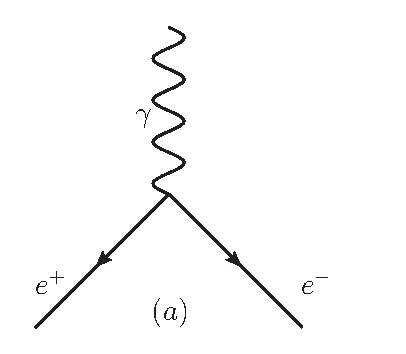
\includegraphics[width=0.3\textwidth]{Chapters/03_Theory/Images/e_e_gamma}\hfill
     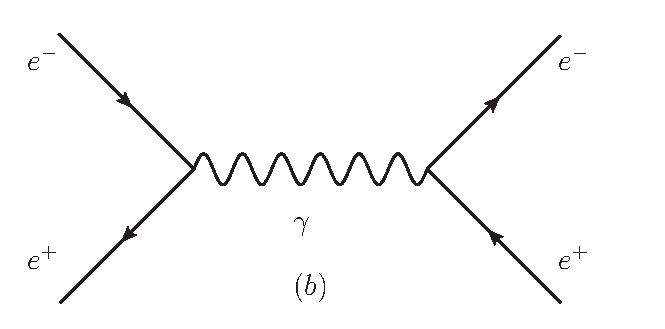
\includegraphics[width=0.5\textwidth]{Chapters/03_Theory/Images/e_e_gamma_e_e}
     \caption[Elementary electromagnetic processes.]{(a) the elementary electromagnetic process of an electron
     emitting a photon and (b) electron-positron annihilation.}
     \label{fig:qed_processes}
\end{figure}

Any such real process is represented by the sum of all possible orders of Feynmann diagrams for a possible
interaction is the representation of the real process. In practice, since at low energies, each vertex
contributes a factor of $\alpha$, higher-order Feynmann diagrams with more than a few vertices contribute
negligibly to the process and are often ignored.

The coupling strength of a force can be further explained in terms of vacuum polarisation. Regarding the
electromagnetic force, this refers to the phenomenon of electron-positron pairs and photons being
spontaneously created and absorbed by an electron. These virtual particles, which would be represented in
Feynmann diagrams as closed loops, shield the original electron leading to the electron charge being measured
at a lower value than its true charge. This measured value is called the effective, or 'screened', charge. As
a result, the coupling strength of the electromagnetic force is said to be a `running' coupling
constant, due to the fact that it decreases as a function of distance.

The mathematical formulation of QED stems from the Dirac equation, which describes the Lagrangian for a
spin-half (Fermionic) field $\psi$~\cite{Dirac610}:

\begin{equation}
\calL = i (\hbar c) \bar{\psi} \gamma^{\mu} \partial_{\mu} \psi - (mc^{2}) \bar{\psi} \psi
\end{equation}

Here, $\hbar$ is the reduced Planck's constant, $\mu$ are the Lorentz indices and $\gamma^{\mu}$ are the gamma
(or Dirac) matrices. Under a global transformation of the field by a phase $i \alpha$,
%\begin{equation}
%\psi(x) \rightarrow \psi'(x) = e^{i\alpha}\psi(x), \bar{\psi} \rightarrow \bar{\psi}'(x) =
%e^{-i\alpha}\bar{\psi}(x)
%\end{equation}
%
this Lagrangian is invariant (\ie under a global transformation of the $U(1)$ group, since this is
equivalent to multiplication of the field $\psi$ by a $1 \times 1$ unitary matrix). However, under a local
gauge transformation by a phase of $i\alpha(x)$, the symmetry %is no longer true since the partial derivative
no longer holds
%\begin{equation}
%\partial_{\mu}(e^{i\alpha(x)}\psi) = i(\partial_{\mu}\alpha(x))e^{i\alpha(x)}\psi +
%e^{i\alpha(x)}\partial_{\mu}\psi ,
%\end{equation}
%
meaning the Lagrangian is not invariant:
\begin{equation}
\calL \rightarrow \calL - \bar{\psi}(x)\gamma^{\mu}\psi(x)[\partial_{\mu}\alpha(x)].
\end{equation}

Local symmetry can be maintained in this case if a new gauge field, $A_\mu$, is introduced to the Lagrangian
by means of a covariant derivative $D_\mu$.%:
%\begin{equation}
%D_{\mu} = \partial_{\mu} + ieA_{\mu}.
%\end{equation}
%
%Under the local transformation, $A_{\mu}$ tranforms as
%
%\begin{equation}
%A_{\mu} \rightarrow A_{\mu}' = A_{\mu} - \frac{1}{e}\partial_{\mu}\alpha(x).
%\end{equation}
%
If the partial derivatives in the Dirac equation are now replaced with the covariant derivatives, the
invariant Lagrangian is obtained:
\begin{equation}
\calL = i (\hbar c) \bar{\psi} \gamma^{\mu} \partial_{\mu} \psi - e \bar{\psi} \gamma^{\mu} \psi A_{\mu} -
(mc^{2}) \bar{\psi} \psi - \frac{1}{4}F^{\mu\nu}F_{\mu\nu}.
\end{equation}

In this way, the principle of local gauge invariance under the $U(1)$ group is used to introduce additional
fields to a Lagrangian in order to make it invariant under local transformations. This final Lagrangian is
that of quantum electrodynamics. The physical interpretation of the gauge field $A_{\mu}$ is the photon, which
couples to charged particles (electrons and positrons) with a coupling strength proportional to the charge.
The term $\frac{1}{4}F^{\mu\nu}F_{\mu\nu}$ is an additional term to account for the kinetic energy of the free
particle of the new gauge field, \ie the photon; and there is no term giving the photon mass.

% \begin{equation}
% F_{\mu\nu} = \partial_{\mu}A_{\nu} - \partial_{\nu}A_{\mu}.
% \end{equation}

\subsection{Electroweak Theory}
\label{ss:electroweak_theory}

The unification of the electromagnetic and weak forces in the 1960s provided a more complete theory of
fundamental particles. This unification takes the form of an $SU(2) \times U(1)$ gauge group combining the
electromagnetic and weak forces, and can be constructed in a similar way to the QED formalism in
Section~\ref{ss:quantum_chromodynamics}.

First, it is necessary to define isospin, $I$, an abstract fundamental property of fundamental particles that
is conserved in all interactions. Similarly, weak hypercharge, $Y$, is also a quantum property, defined as
$Y_{W} = 2(Q-I_{3})$, where $Q$ represents the charge of the particle and $I_{3}$ is the third component of
isospin. $I_{3}$ takes a value of $1/2$ for left-handed fermions.

It has been shown empirically that the weak interaction exhibits violation of parity ($P$) and interacts only
with left-handed particles via the charged gauge bosons ($\W^{\pm}$). Hence, the fields representing fermions
are split into left handed and right handed components by defining a left handed doublet containing the left
handed electron and left handed neutrino, and a right handed singlet containing the right handed electron.%:
% \begin{equation}
% \chi_{L} = \left( \begin{array}{c} \nu_{e} \\ e \end{array}\right)_{L}, e_{R}
% \end{equation}
% Here, the left handed doublet has $I=\frac{1}{2}$, and the right handed lepton has $I = 0$. Similar doublets
% can be constructed for the other generations of leptons ($\mu$ and $\tau$) and quarks in their pairs of three
% generations ($\cPqu\cPqd$, $\cPqc\cPqs$ and $\cPqt\cPqb$). Right handed neutrinos, which would have $I=0$ and
% $Y=0$, do not exist in the Standard Model. %as they would not interact with any of the force mediators.

Four additional massless fields and their associated currents are introduced in order to impose
gauge-invariance: $\W_{\mu}^{1}$, $\W_{\mu}^{2}$, $\W_{\mu}^{3}$ and $B_{\mu}$. The $\W_{\mu}$ fields are
introduced for gauge invariance of the $SU(2)$ group, and interacts with the third isospin component $I_{3}$.
The $B_{\mu}$ field similarly transforms by the unitary group $U(1)$, and interacts with the weak hypercharge
$Y$. These additional fields lead to the construction of three weak isospin currents and a weak hypercharge
current.

Requiring local gauge invariance under a $SU(2) \times U(1)$ group, the covariant derivative is
\begin{equation}
D_{\mu} = \partial_{\mu} + \frac{i}{2} g_{\W} \vec{\tau} \cdot \vec{\W}_{\mu} + ig' \frac{Y}{2}B_{\mu}.
\end{equation}

The vectors $\W_{\mu}^{1}$, $\W_{\mu}^{2}$, $\W_{\mu}^{3}$ have coupling strengths of $g_{\W}$ to the three
isospin currents and $B_{\mu}$ couples to the hypercharge current with a strength of $g'$. These four bosons
relate to the quanta of the new fields. A linear superposition of the $\W_{\mu}^{1}$ and $\W_{\mu}^{2}$ states
gives the $\W^{\pm}$ bosons, while the neutral states $\W_{\mu}^{3}$ and $B_{\mu}$ undergo a mixing related by
the weak mixing angle, $\theta_{\W}$, to give the neutral $\Z^{0}$ and $\gamma$ bosons. (The weak mixing angle
relates the coupling constants of the electromagnetic and weak forces by $\tan \theta_{W} =
\frac{g'}{g_{W}}$).

It has been experimentally observed that both the \W bosons and the \Z boson have mass. Indeed, the
strength of the electromagnetic force is of the same order as the weak force, but as a result of the weak
gauge bosons having mass, the weak force appears weaker and has a shorter range. However, the local gauge
invariance would be broken if terms are now included to give the bosons mass. The theory of spontaneous
breaking of the symmetry underlying the $SU(2) \times U(1)$ group addresses this problem, as explained in
Section~\ref{ss:spontaneous_symmetry_breaking}.

The weak force has been shown to change the flavour of quarks in an interaction, meaning flavour conservation
is broken. %As stated,
The quarks, like leptons, come in the form of left handed doublets within each generation,
\begin{equation}
\left(\begin{array}{c} u_{L} \\ d'_{L} \end{array}\right) , \left(\begin{array}{c} c_{L} \\ 
s'_{L} \end{array}\right) , \left(\begin{array}{c} t_{L} \\ b'_{L} \end{array}\right)
\end{equation}
with isospin $\frac{1}{2}$. Note that the lower quarks of the doublets are denoted with primes as they
indicate a rotated state of the quark, called Cabibbo-rotated states, which are superpositions of the physical quarks.
This means that in, for example, the decay of a down quark to an up quark via emittance of a $\W^{-}$, the
down quark to which the $\W^{-}$ couples is actually a superposition of `down type' quarks, \ie down, charm
and beauty quarks. The Cabbibo-Kobayashi-Maskawa (CKM) matrix, relates the weak interaction mixed states to
the physical quark states. This is the degree of quark mixing between the different generations, and results in
the measured values (see equation~\ref{CKM_matrix}) of $\abs{V_{12}}$ for the probability of a transition from
quark 1 to quark 2 in a weak interaction~\cite{Agashe:2014kda}. In reference to top physics, the \abs{V_{tb}} value of almost 1
means that the top quark almost always decays to a \W boson and a \bquark.

\begin{equation}
\begin{pmatrix}
V_{\cPqu\cPqd} & V_{\cPqu\cPqs} & V_{\cPqu\cPqb} \\
V_{\cPqc\cPqd} & V_{\cPqc\cPqs} & V_{\cPqc\cPqs} \\
V_{\cPqt\cPqd} & V_{\cPqt\cPqs} & V_{\cPqt\cPqb} 
\end{pmatrix}
=
\begin{pmatrix}
0.974 & 0.225 & 0.004 \\
0.225 & 0.973 & 0.041 \\
0.009 & 0.041 & 0.999
\end{pmatrix}
\label{CKM_matrix}
\end{equation}

\subsection{Quantum Chromodynamics}
\label{ss:quantum_chromodynamics}

In the theory of quantum chromodynamics (QCD), the charge of the strong force is colour, and the force is
independent of other particle properties such as charge and flavour. Empirical data has led to the conclusion
that there are three colour charges: red, green and blue~\cite{Griffiths:1987tj}. Colour conservation is a
requirement of strong processes (cf. charge conservation in QED), although the colour of an individual quark
can be changed in a strong interaction. The mediators of the strong force, gluons, carry a positive and a
negative colour charge themselves, and so can interact directly with other gluons. The coupling constant of
the strong force is a running coupling constant. At small distances of the order of the size of the proton
(\textasciitilde0.1\fm), $\alpha_{S}$ is small and becomes smaller as distance decreases, leading to quarks
and gluons being essentially free particles and interacting weakly with each other when confined within
colourless bound states (though this interaction is still stronger than the electromagnetic force). This
phenomenon is termed asymptotic freedom.

The previously mentioned colourless bound quark states are called hadrons. The process in which free gluons
and quarks form bound colourless states is called hadronisation, and at high momenta manifests as a cone of
particles, termed jets. Hadrons are divided into two types: mesons are composed of a quark and an antiquark
with the quark carrying a colour charge and the antiquark carrying the respective anticolour; baryons are
composed of three quarks or three antiquarks. Recently, the LHCb experiment at CERN published first results of
the observation of a pentaquark state~\cite{Aaij:2015tga}.

The proton, a baryon, consists of two \uquarks, one \dquark and gluons binding the quarks together. However,
the structure of the proton becomes more complicated, consisting of more particles, as the momentum of the
probing particle increases. The aforementioned three-quark-structure of the proton is evident at low momenta,
while at higher momenta, virtual pairs of quarks, antiquarks and gluons are visible. These virtual quarks and
gluons are termed sea quarks and can make up most of the mass of the proton at high energy scales. In any
proton, each constituent particle carries some fraction, $x$, of the overall proton momentum.

The quantum field theory of QCD is determined to have the underlying symmetry of the group $SU(3)$, based on
the fact that there are three colour charges. Imposing local gauge invariance, the Lagrangian contains eight
generators of the $SU(3)$ group. These generators lead to eight gauge fields, whose physical interpretation
are the eight massless gluons that mediate the strong force. Therefore, although in principle there could be
nine gluons, since there are three colours and gluons carry a colour and an anticolour charge, the $SU(3)$
symmetry leads to a colour octet and a colour singlet~\cite{Griffiths:1987tj}.

Any particle that occurs in nature must be a colour singlet, and so the gluons in the colour octet are never
seen in nature. However, although the final gluon is a colour singlet, it has not been observed and is
thought not to exist. If it did exist, it would result in a long range strong force, but it is known that the
strong force has a short range of action.

\subsection{Spontaneous Symmetry Breaking}
\label{ss:spontaneous_symmetry_breaking}

The theory of spontaneous breaking of the electroweak $SU(2)$ symmetry, mentioned in
Section~\ref{ss:electroweak_theory}, also known as the Higgs mechanism, was put forward in the
1960s~\cite{Higgs:1964pj}. This theory was postulated as a mechanism by which the $\W^{\pm}$ and \Z gauge
bosons could acquire mass, since the Lagrangian of the electroweak interaction contains no mass term for these
particles, and their inclusion would violate local gauge invariance.

The method by which this symmetry is spontaneously broken begins with the inclusion of two new complex scalar
`Higgs' fields (so in total there are four components to these two complex fields). These fields are
introduced with an additional scalar potential energy term in the Lagrangian, $V(\Phi)$, where $\Phi$
represents the newly introduced complex scalar fields. %in the form of a doublet.
The potential $V(\Phi)$ is chosen to be
\begin{equation}
V(\Phi) = -\mu^{2} \Phi^\dagger \Phi + \lambda^{2} (\Phi^\dagger \Phi)^{2}
\end{equation}
Imposing the requirement of $\mu^{2}$ and $\lambda$ both being greater than 0, gives a potential of the
geometry shown in Figure~\ref{fig:higgs_potential}. The minimum of this potential is clearly not at
$\Phi=0$, rather, the minimum has a circular form given by the formula $\Phi^\dagger \Phi =
\frac{\mu^{2}}{2\lambda} = \frac{v^{2}}{2}$, where $v = \frac{\abs{\mu}}{\sqrt\lambda}$, the `vacuum
expectation value' of the Higgs field. Since the minimum, \ie the vacuum, is at a location other than $\Phi =
0$, the new field is said to have a non-zero vacuum expectation value, and the $SU(2) \times U(1)$ symmetry is
spontaneously broken. The observed Higgs boson is created as a result of perturbations in the potential about
this minimum. % which removes three of the four $\Phi$ components as the \W^{+}, \W^{-} and \Z bosons, with
% the remaining field being the scalar Higgs field.
In addition to this new particle, introducing the new fields also results in the fields associated with the
$\W^{\pm}$ and $\Z^{0}$ bosons in the Lagrangian acquiring mass.
%One of these new fields, $\eta$ and $\xi$. One of these, known as the Goldsone boson, is eaten by the other
%thereby acquiring mass. It is this field that is known as the Higgs field.

\begin{figure}[hbtp]
   \centering
     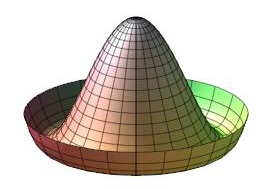
\includegraphics[width=0.5\textwidth]{Chapters/03_Theory/Images/higgspot}\hfill
     \caption[The Higgs field potential.]{The Higgs field potential $V(\Phi)$~\cite{Moss:2015fma}.}
     \label{fig:higgs_potential}
\end{figure}

Terms known as Yukawa coupling terms can be introduced to specify the interactions of $\Phi$ with the fermion
fields. It is this coupling of the Higgs field to any massive particle that gives them a proportional mass.
The top quark, being the heaviest known particle at \textasciitilde173\GeV, has a Yukawa coupling to the
Higgs field close to 1.
%TODO: IMPORTANT BECAUSE?

Results published at the discovery of the Higgs boson are shown in Figure~\ref{fig:higgs_results} in the
Higgs$\rightarrow\gamma\gamma$ and Higgs$\rightarrow\Z\Z$ channels. These plots of the invariant masses of the
$\gamma\gamma$ and $\Z\Z$ combinations show a clear excess of events around 125\GeV. The latest results from
CMS and ATLAS state a Higgs mass of $125.09\pm0.21\pm0.11\GeV$~\cite{Aad:2015zhl}, where the first uncertainty
is statistical and the second is systematic. Since the announcement of the discovery of the Higgs boson in 2012,
studies have continued to determine its quantum properties. Thus far, results show it to be in agreement with
predictions from the Standard Model.

\begin{figure}[hbtp]
   \centering
     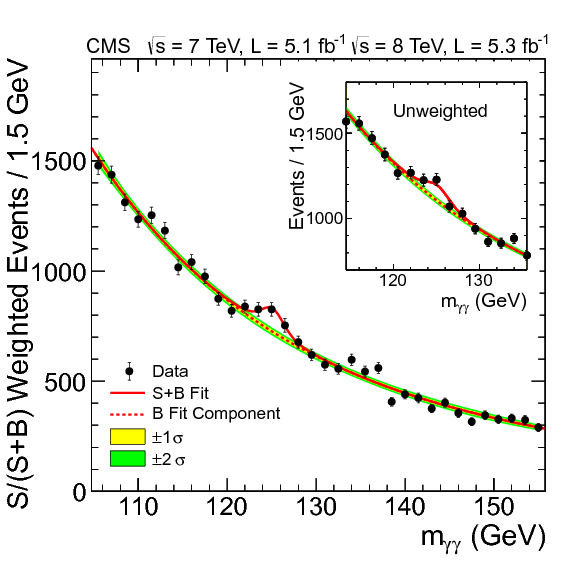
\includegraphics[width=0.5\textwidth]{Chapters/03_Theory/Images/sbweightedmassunweightedinset1_5GeV}\hfill
     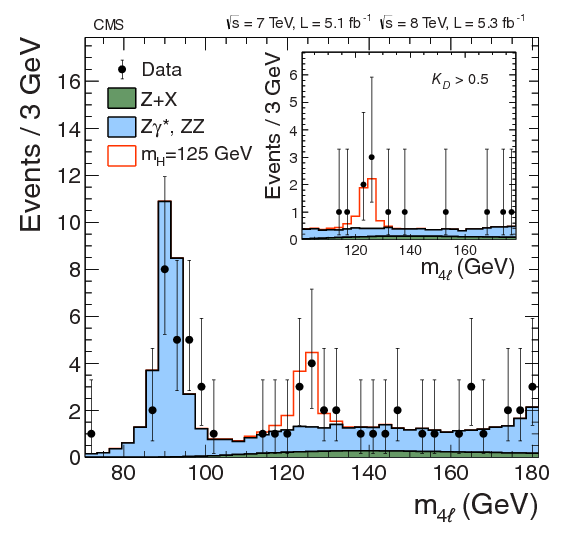
\includegraphics[width=0.5\textwidth]{Chapters/03_Theory/Images/H4l_mass_v3}\hfill
     \caption[Invariant mass in $H\rightarrow\gamma\gamma$ (left) and $H\rightarrow\Z\Z$ (right)
     channels.]{Invariant mass in $H\rightarrow\gamma\gamma$ (left) and $H\rightarrow\Z\Z$ (right) channels
     ~\cite{Chatrchyan:2012xdj}.}
     \label{fig:higgs_results}
\end{figure}

\section{Incompleteness of, and physics beyond, the SM}
\label{s:Incompleteness_of_and_physics_beyond_the_SM}
The Standard Model has proven to be an extremely successful theory thus far. However, its inability to
describe many phenomena in the universe lead to it being considered currently incomplete. Indeed, a `Grand
Unified Theory' combining the electromagnetic, weak and strong interactions is considered to be the next step
towards a `Theory of Everything' including gravity, with all of these forces being different physical
manifestations of one single force.

There are many free parameters in the Standard Model and the very reason why it takes the form it has, with
four fundamental forces, six quarks and six leptons, each divided into three generations, is not explained.
The gravitational force is also conspicuous by its absence from the SM. The imbalance between matter and
anti-matter in the universe, despite the generally accepted view that both were created in equal quantities in
the Big Bang, is also not fully explained by the SM. Although the evident matter-antimatter asymmetry in the
unvierse could be partially explained by the observed charge-parity (CP) symmetry violation in weak
interactions~\cite{Christenson:1964fg}, this is not sufficient to account for the observed excess.

Furthermore, the SM does not provide a theoretical explanation for neutrino mass. Originally thought to be
massless, neutrinos are now thought to have mass, albeit extremely small, based on observations of neutrino
oscillations between different flavours~\cite{Kajita:1998bw,Fukuda:1998mi}.

The hierarchy problem, in terms of the Higgs boson, refers to the fact that the measured Higgs mass is many
orders of magnitude smaller than the order of the Planck scale ($1.22\times10^{19}\GeV$). The expected
quadratically divergent quantum corrections to the Higgs mass from higher order interactions should result in
a far higher mass. This disagreement suggests that there occurs some `fine tuning' of the bare Higgs mass, to
lead to the experimentally observed mass of approximately 125\GeV.

Supersymmetry (SUSY) is one potential solution to hierarchy problem. This theory proposes a symmetry between
fermions (spin $\frac{1}{2}$) and bosons (spin 1). Each particle has an associated `superpartner' with
identical quantum properties with the exception of spin, which differs by $\frac{1}{2}$, so that all SM
fermions have a boson superpartner, and all SM bosons have a fermion superpartner.
These super particles, or sparticles, are thought to have higher masses than their SM counterparts since they
have not been discovered yet, making supersymmetry a broken symmetry. In many supersymmetry theories, the
lightest SUSY particle (LSP) is stable and is a potential candidate to be a dark matter particle.

Another potential solution is the theory of topcolor, an example of a composite model theory that suggests the
existence of a top-quark-condensate (a composite field of the top and antitop
quarks)~\cite{1990PhRvD..41.1647B,1991PhLB..266..419H} that acts effectively like the SM Higgs field. Such a
theory gives rise to a new fundamental interaction between top quarks at high energies resulting in the large
top mass. Theories of extra dimensions also exist, in which additional space-time dimensions are postulated in
which only gravity propagates~\cite{ArkaniHamed:1998rs}.
This could provide an explanation for the fact that the Planck scale is far larger than the electroweak force
by solving the heirarchy problem.

The universe is thought to constitute of about 27~\% dark matter, 68~\% dark energy and 5~\% ordinary
matter (Figure~\ref{fig:universe_composition})~\cite{Ade:2013sjv}. The origins and nature of the dark energy and dark
matter are currently unknown and they are as yet unobserved, but their existence has been inferred from their
gravitational effects on galactic masses composed of stars, gases and dust. The relatively large amounts of
dark matter and dark energy hypothesised suggests that they are made up of weakly interacting massive
particles.

\begin{figure}[hbtp]
   \centering
     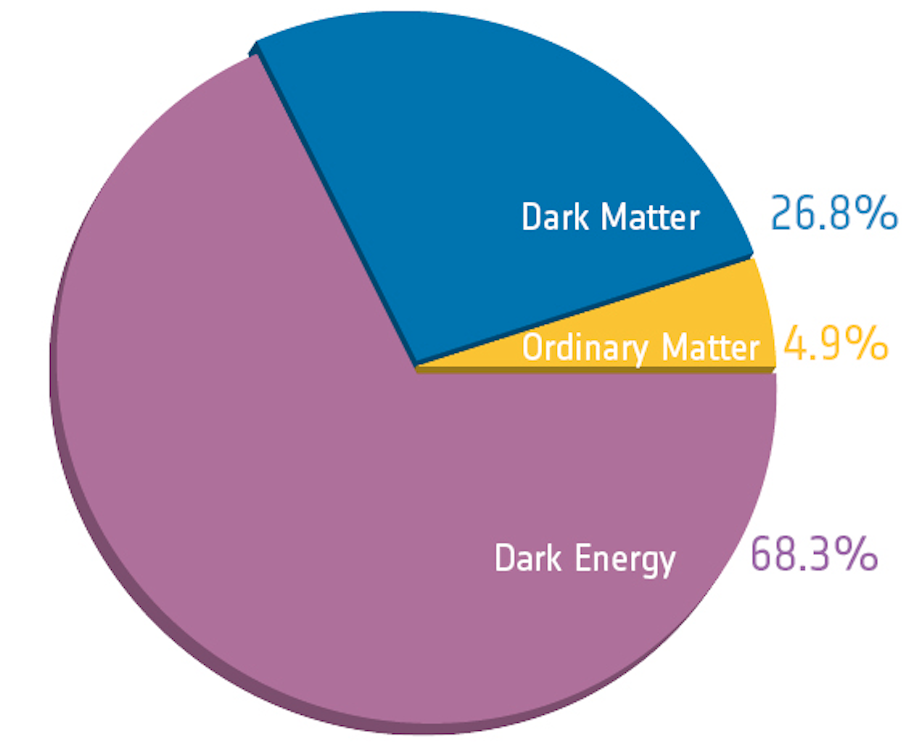
\includegraphics[width=0.5\textwidth]{Chapters/03_Theory/Images/planck_cosmic_pie}\hfill
     \caption[The composition of the universe showing the amounts of dark matter, dark energy and ordinary
     matter.]{The composition of the universe showing the amounts of dark matter, dark energy and ordinary
     matter based on latest results from Planck/ESA~\cite{Ade:2013sjv}}
     \label{fig:universe_composition}
\end{figure}
